RF (radio frequency) based ranging problem is concerned with inferring distance between two agents/robots in space using radio antennas.

The chapter is divided in a following way: first describing general methods of measuring distance between two RF devices/antennas, secondly investigating existing protocols making measurements and lastly selecting a technology for later implementation of positioning system based on ranging technology.

Requirements for application:
\begin{itemize}
    \item Long range - preferably up to 100m or more (so that agent can cover bigger area).
    \item High precision - accuracy of at least 10cm at short distances (in order to avoid collisions whenever two agents would be close to each other).
    \item Measurement frequency of at least 10Hz or more (this allows agent to execute faster trajectories).
\end{itemize}

\subsection{Range measurement methods}

Literature points out two main methods for making distance measurements over RF antennas: RSSI (Received Signal Strength Indication) and time based methods. There is also approaches based on angle of arrival (AoA) but it's not explored here.

\subsubsection{RSSI}

As the name suggests the received signal strength hints at the power of incoming radio signal. There is non-linear corelation between RSSI and distance between two antennas \cite{rssi-curves}:
$$
    R S S I=-10 n \log _{10}(d)+C
$$
thus it is possible, for instance, to fit a curve on a measured experimental values like shown in \cite{rssi-curves}. However, the main disadvantage that for commercial protocols the quantity over distance curve flattens out at certain distance and further it's impossible to tell the a difference between different measurements. The effect can be seen in Figure \ref{fig:rssi-curves} for indoor applications (meaning having obstacles in a path). The figure shows plots of RSSI vs Distance plots for different protocols like WiFi, BLE, etc.

Also in \cite{blerssi} authors provide line-of-sign scenario results of BLE and WiFi RSSI from a commercial phone. Figure \ref{fig:sec-rssi-curves} shows their results on measuring RSSI multiple times i.e. data is collected at different times. The variation between different BLE data points is relatively huge and influences range accuracy is a significant way. Both BLE and WiFi curves flatten out as distance is increasing and it's evident that above certain limit signal strength is not usable as a viable distance measurement. Also there is quite a bit of variation, curves are not smooth so the precision of data points is quite low.
\begin{figure}[H]
    \centering
    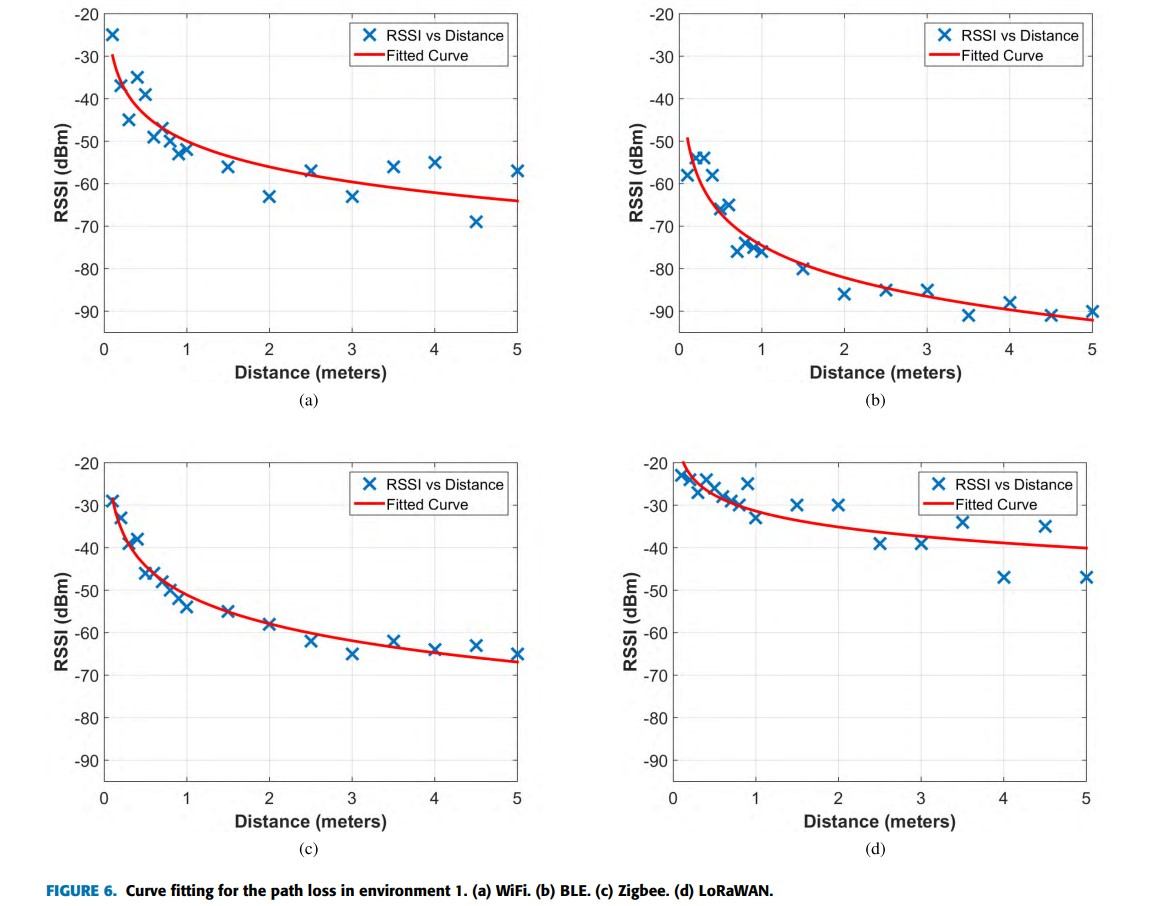
\includegraphics[width=.8\linewidth]{figures/RSSICurves.jpg}
    \caption{Various protocol RSSI over distance curves \cite{rssi-curves}.}
    \label{fig:rssi-curves}
\end{figure}
\begin{figure}[H]
    \centering
    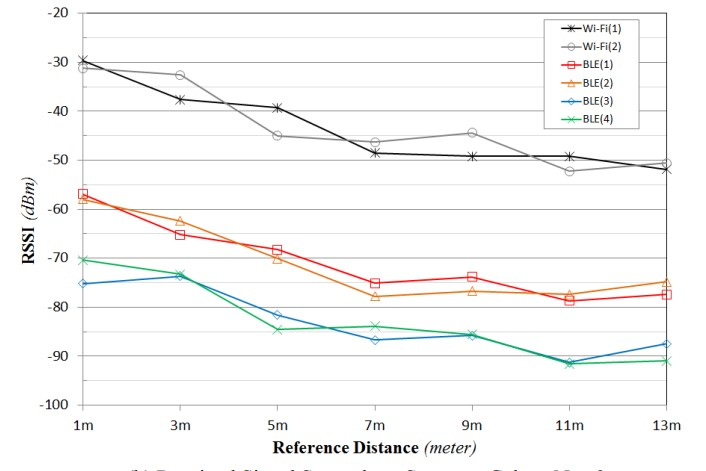
\includegraphics[width=.7\linewidth]{figures/blesrri.jpg}
    \caption{BLE RSSI curve on  Samsung Galaxy Note3 \cite{blerssi}.}
    \label{fig:sec-rssi-curves}
\end{figure}

\subsubsection{Time based}

These methods are based on measuring radio wave propagation time between (or ToF - \emph{Time of Flight}) antennas/devices and calculating the distance by knowing light speed i.e. $d=ct$, where $c=3 * 10^{8}$ m/s. One obvious drawback here is that two clock must be synchronized if to infer the distance by ToA (\emph{Time of Arrival}). However, this can be avoided by doing a round trip (in literature referred as TDoA - \emph{Time Difference of Arrival}) and relying solely on one clock. The scheme is illustrated in \ref{fig:RTT} where $T_{prop}$ is propagation time in which we are interested in for ranging applications. The value can be computed by $T_{prop} = \frac{1}{2}(T_{round} - T_{reply})$. Also, Figure \ref{fig:RTT} correctly indicates the scale of $T_{round}$ and $T_{prop}$. Important thing to notice here, if the distances we're measuring are in order of meters, $T_{prop} = d/c$ evaluates to nanosecond scale while for response computer might have to execute hundreds of instructions taking up way more time than the time we're interested in. Thus it's of most importance to know how much time computation takes in the responding device. When selecting/designing a system to use RTT for positioning, responding device must have very fine granularity control of computing resources. If one would try to make these computations on OS (Operating system) level, the time jitter introduced by OS scheduling system would be so large that propagation time would vanish in the error of $T_{reply}$ measurement.
\begin{figure}[H]
    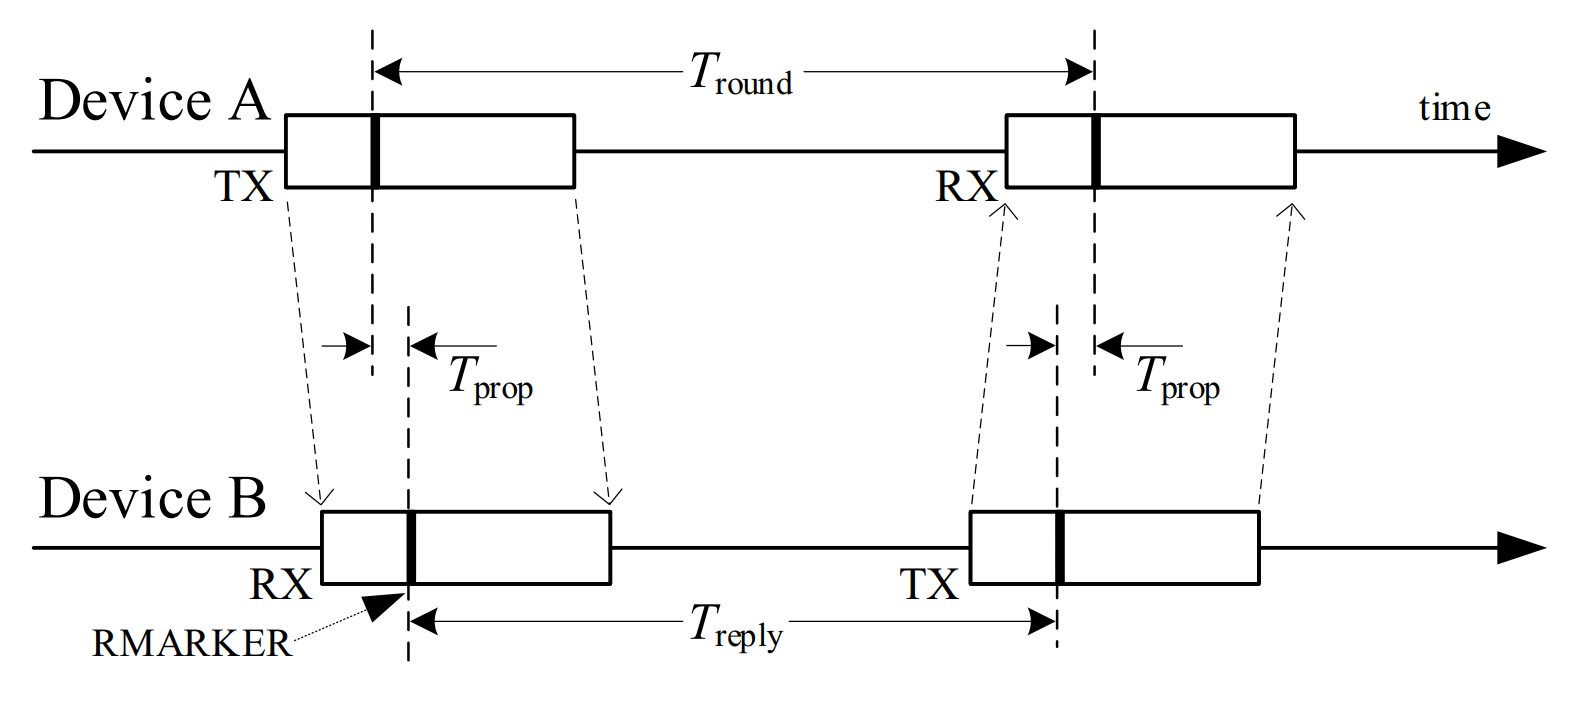
\includegraphics[width=\linewidth]{figures/RTT.jpg}
    \caption{Round trip time \cite{9179124}.}
    \label{fig:RTT}
\end{figure}

\subsection{RF positioning}

There are many existing protocols/technologies to exchange data between devices over the air i.e. by transmitting it over electromagnetic waves. In this chapter, a few of most popular ones will be reviewed in terms of how suitable each of them is for positioning applications. WiFi, UWB (Ultra Wide Band) and BLE (Bluetooth Low Energy) protocols are investigated.

All of the below described protocols do support RSSI ranging (by the nature of them being radio communication the signal strength assessment can always be made) but due to limitations the focus is on on time based ranging methods to fulfill the application requirement with selected technology.

Although conceptually calculating distance from time it took to traverse the space for a radio wave is very simple, implementing it in reality is very difficult because time stamping must be done at a hardware level to have reasonable precisions when distance equation involves light speed. For instance, $1 \mu s$ corresponds to $300m$ difference in distance measurement. Thus significant effort is spent to develop standard protocols and techniques to make this work in practice.

\subsubsection{WiFi}

\emph{IEEE 802.11-2016} standard includes a Fine Time Measurement (FTM) protocol for WiFi ranging technique. This allows very granular measurement of time, enabling time-stamping WiFi transmissions (obtaining RTT) precise enough to calculate distances between devices. However hardware support is very limited even for high-end WiFi products.

Even with specialized (expensive) hardware this approach requires quite a bit of effort to install required driver, firmware, kernel version. The distance measurement is also not that precise - best case scenario gives $1-2m$ accuracy.

For instance, in paper \cite{ibrahim2018verification} authors were able to make it work while getting mentioned accuracy and collecting data point from devices up to couple hundred meters apart. Nevertheless, the used hardware is not readily available for purchase (they mention a chip used, but quick internet search doesn't give any practical answers where to buy antenna with the exact chip on it) or requires one to buy full router (costing hundreds of dollars for each device).

\subsubsection{BLE}

BLE protocol is widely supported and available even on low-end cheap devices like Arduino microcontroller. The main problem is that no standard way of measuring RTT is present in the protocol thus the only only option to get a range measurement is to use RSSI which was already discussed as not suitable for the application/requirement of the project.

\subsubsection{UWB}

UWB is one of the most widely used radio technology for positioning applications because of the wide support for for range measurement and existing protocols to do that. Many chips sets are present on market with off the shelf distance measurement capabilities (like DW1000 \cite{dw1000chip} or U1 in Apple products). This shows the extent to which technology is matured enough to be used in real-world applications.

Standard IEEE Std 802.15.4z-2020 \cite{9179124} specifically defines ranging techniques that can be readily implemented in hardware and software of UWB supporting microcontrollers. Method described in the standard is based on RTT with additional measures to increase robustness and precision in practical implementations. However, in essence round trip time approach is selected because of no need to calibrate the clocks on devices and if time measurements are done in a precise way the distance calculation is very straightforward.

Due to convenience, availability and other properties that meets the requirements UWB based ranging is select to be used in special course positioning experiments as most suitable protocol.

\subsection{Other}

There are many RF communication protocols that might be promising for positioning applications. For example, LoRa has potential in long-range low-accuracy positioning application or 5G could be also be considered as alternative approach with similar performance to UWB although not that widely adopted yet. However, these were not investigated in detail here.